\documentclass[../main.tex]{subfiles}
\graphicspath{{\subfix{../images/}}}

\begin{document}
\newcolumntype{C}{>{\centering\arraybackslash}p{0.3\textwidth}}

\subsection{Πεδία Ορισμού}

\renewcommand{\arraystretch}{1.5}
\tymin 0.3\textwidth
\begin{table}[H]
	\centering
	\begin{tabular}{C|C}
		\hline
		\textbf{Πεδίο ορισμού} & \textbf{Τύπος} \\
		\hline
		ταυτότητα              & INT(4)         \\
		ημερομηνία             & DATE()         \\
		όνομα                  & VARCHAR(25)    \\
		αλφαριθμητικό          & VARCHAR(25)    \\
		προσδιορισμός          & ENUM()         \\
		συντεταγμένες          & REAL()         \\
		\hline
	\end{tabular}
	\caption{Πεδία ορισμού της βάσης got-db}
\end{table}


\newenvironment{relation}[1]
{\renewcommand{\arraystretch}{1.4}
	\newcommand{\temp}{#1}
	\begin{table}[H]
		\centering
		\begin{tabular}[t]{*{2}{C}}
			\hline
			\multicolumn{2}{c}{Όνομα Σχέσης: \bf{#1}} \\
			\hline
			\multicolumn{2}{c}{\bf{Γνωρίσματα}}       \\
			\hline
			\textbf{Όνομα} & \textbf{Τύπος}           \\
			}
			{
			\hline
		\end{tabular}
		\caption{Σχέση \texttt{\temp}}
	\end{table}
}

\subsection{Σχέσεις}

\begin{relation}{character}
	character\_id         &  ταυτότητα\\
	name                  &  όνομα \\
	alias                 &  προσδιορισμός \\
	date\_of\_birth       &  ημερομηνία \\
	date\_of\_death       &  ημερομηνία \\
	titles                &  αλφαριθμητικό \\
\end{relation}

\begin{relation}{house}
	slogan                &  αλφαριθμητικό\\
	house\_name           &  όνομα \\
\end{relation}

\begin{relation}{non human}
	ID                &  ταυτότητα \\
	name              &  όνομα \\
	species           &  αλφαριθμητικό \\
\end{relation}

\begin{relation}{notable events}
	date              & ημερομηνία \\
	nickname          & όνομα \\
	Type\_of\_event   & προσδιορισμός \\
	outcome           & προσδιορισμός \\
\end{relation}

\begin{relation}{religion}
	name & όνομα \\
\end{relation}

\begin{relation}{location}
	x     & συντεταγμένες \\
	y     & συντεταγμένες \\
	name  & όνομα \\
\end{relation}

\subsection{Σχεσιακό Σχήμα}

\begin{figure}[H]
	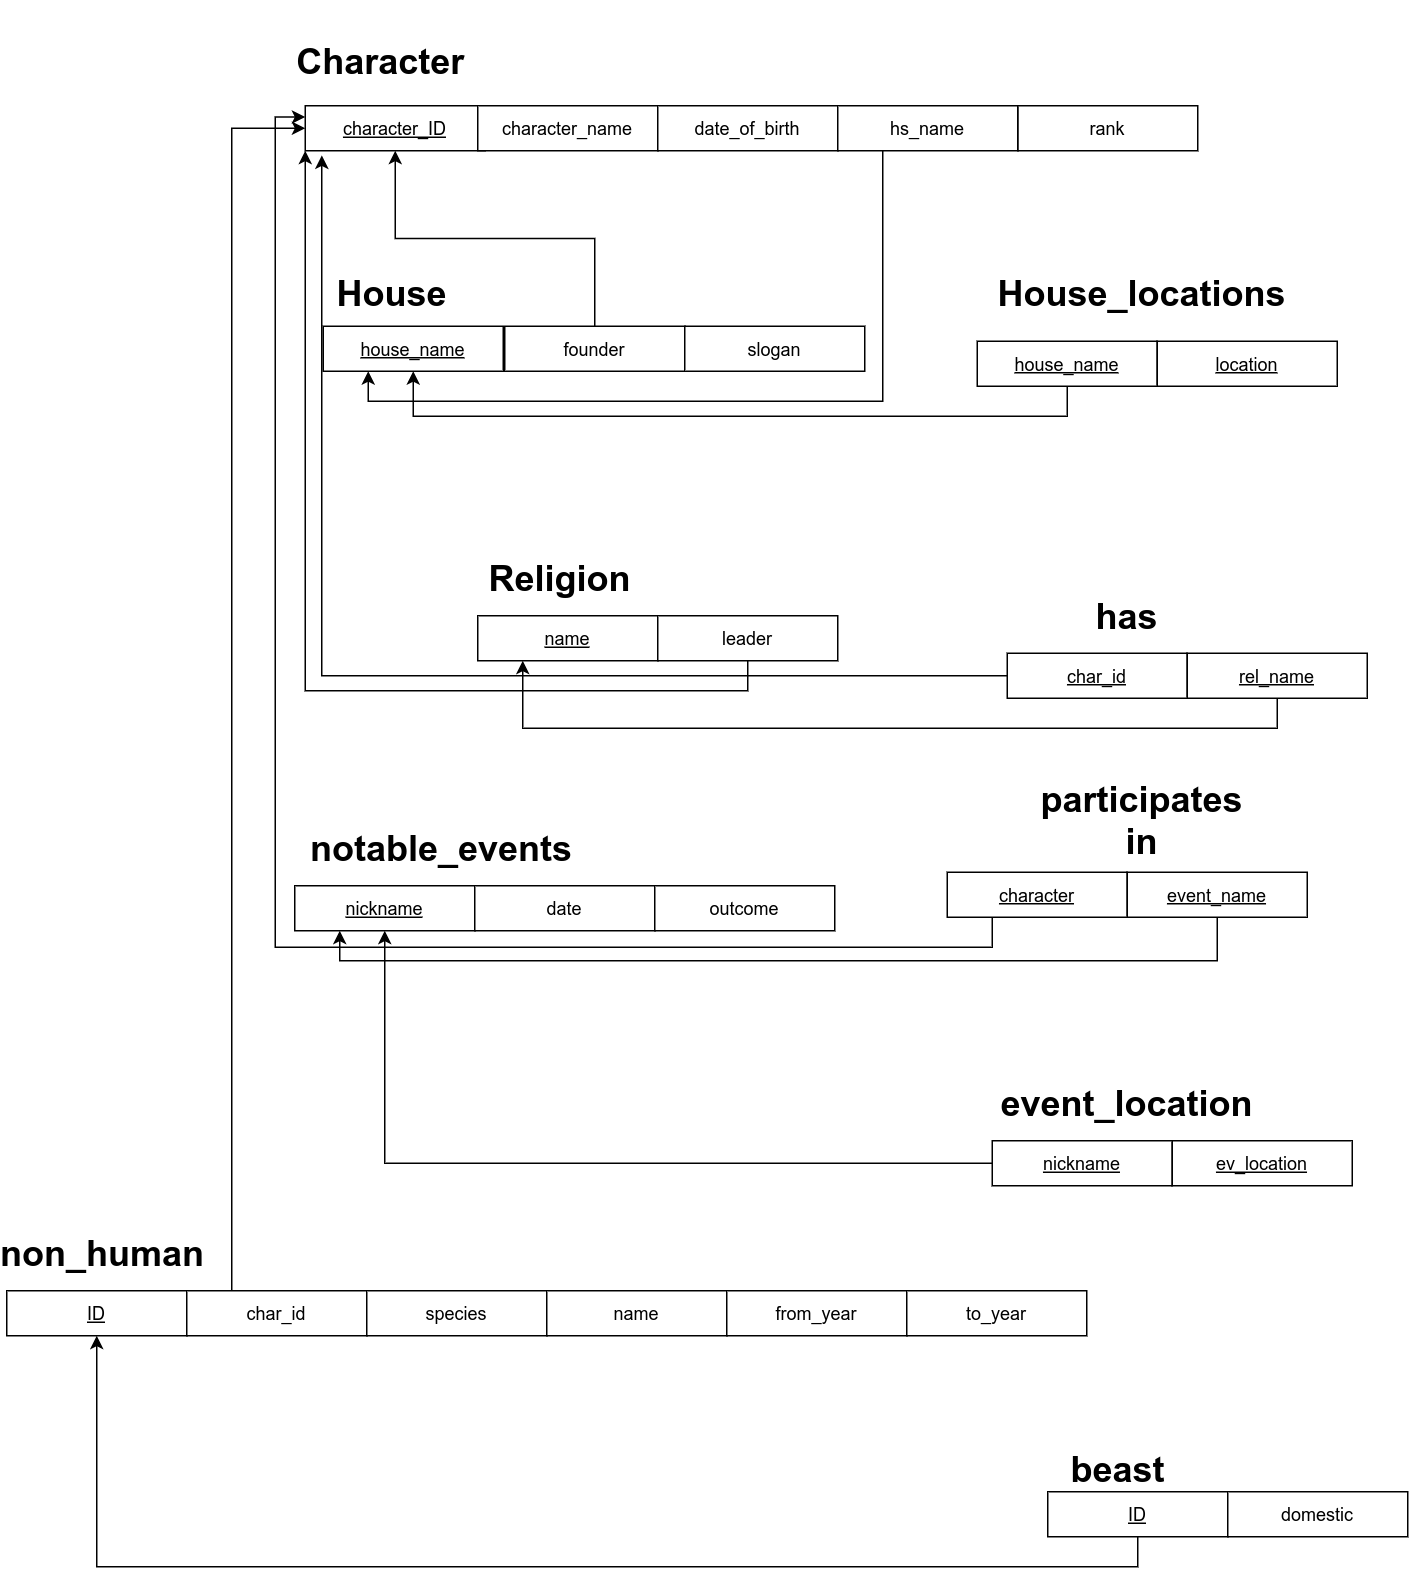
\includegraphics[width=\textwidth]{../images/relation_diagram.png}
	\caption{Σχεσιακό Σχήμα}
\end{figure}

\subsection{Όψεις}

% command for smaller subscripts

\noindent
Όψη που περιέχει όλους τους ηγέτες οίκων και τα ονόματα των οίκων
αυτών.
\begin{figure}[H]
	\begin{equation}
		\bm{\rho}_{\tsub{LEADERS}}
		(
		\bm{\pi}_{\tsub{c.char\_id,c.house\_id,c.Character,h.name}} (
		\bm{\rho}_{\tsub{c(char\_id,Character)}}(\texttt{characters})
		\bowtie_{\tsub{h.id=c.house\_id}}
		\bm{\rho}_{\tsub{h}}(\texttt{houses})
		))
	\end{equation}
	\caption{Όψη leaders}
\end{figure}

\noindent
Όψη που περιέχει όλα τα μην αν ανθρώπινα όντα που ανήκουν σε κάποιον
χαρακτήρα.
\begin{figure}[H]
	\begin{equation}
		\begin{aligned}
			\bm{\rho} & _{\tsub{OWNED\_NON\_HUMANS}} (               \\
			          & \bm{\pi}_{\tsub{nh.id,nh.name,nh.species}} (
			\bm{\rho}_{\tsub{nh}}(\texttt{non\_humans})
			\bowtie_{\tsub{nh.id=cnh.non\_human\_id}}
			\bm{\rho}_{\tsub{cnh}}(\texttt{character\_non\_human})
			))
		\end{aligned}
	\end{equation}
	\caption{Όψη non\_humans\_with\_owners}
\end{figure}

\noindent
Όψη που περιέχει τους χαρακτήρες που πιστεύουν σε κάποια θρησκεία μαζί με το
όνομα της θρησκείας.
\begin{figure}[H]
	\begin{equation}
		\begin{aligned}
			\bm{\rho} & _{\tsub{characters\_with\_religions}} (                                                                                                     \\
			          & \bm{\pi}_{\tsub{c.char\_id, r.rel\_id, c.Character, r.Religion}} (                                                                          \\
			          & \quad(\bm{\rho}_{\tsub{c}}(\texttt{characters}) \bowtie_{\tsub{c.id=cr.character\_id}} \bm{\rho}_{\tsub{cr}}(\texttt{character\_religion})) \\
			          & \quad\bowtie_{\tsub{r.id=cr.religon\_id}}                                                                                                   \\
			          & \quad\ \bm{\rho}_{\tsub{r}}(\texttt{religions})                                                                                             \\
			          & ))
		\end{aligned}
	\end{equation}
	\caption{Όψη characters\_with\_religions}
\end{figure}


\end{document}
